\documentclass{beamer}
\usepackage[utf8]{inputenc}
\usepackage{graphicx}

% themes found here: https://latex-beamer.com/tutorials/beamer-themes/
% \usetheme{PaloAlto}
\usetheme{CambridgeUS}
\setbeamertemplate{footline}[frame number]

\title{Resilient Weather Interpolation}

\author{
    Baxter, Hunter %\\
    \and
    Callandriello, Meghan
    \and
    Hicks, Jaden
    \and
    Pena, Alex
}

\begin{document}
\maketitle

\begin{frame}{Main Idea}
\begin{itemize}
    \item The goal of our project is less about creating a novel solution to an unsolved problem,
    but rather utilizing \textbf{industry grade} tools on a small scale
    % spatio-temporal data has sweet visualizations so it offers something to everyone
    \item The data we will be working with is \textbf{spatio-temporal}
    % acknowledge that this is just a demonstration of spatio-temporal data, not that weather is a cutting edge problem
    \item The objective is to \textbf{fill sparsity} of data over a geographic region in a hypothetical situation where there is a scarcity of sensors \textbf{due to some constraint}
    % mention why real time weather data matters (ex. road conditions, agriculture) 
\end{itemize}
\end{frame}

\begin{frame}{Architecture}
\begin{center}
    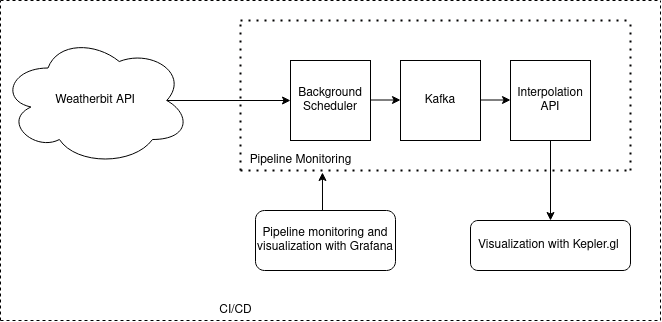
\includegraphics[width=\linewidth]{figures/architecture.png}
\end{center}
\end{frame}

\begin{frame}{Resilient?}
\begin{columns}
    \begin{column}{0.5\textwidth}
    \begin{itemize}
        \item A system is defined as \textbf{resilient} if it continues to carry out its mission in the face of adversity
        % \item Although we can not achieve or guarantee perfect resiliency, we can employ strategies to enhance it
        \item \textbf{Kafka} ensures correct delivery of messages
        % kafka: at least once delivery 
        % indempotent producer
        % we should have more than one broker
        \item \textbf{Kubernetes} ensures redeployment in case of failures
        % TODO: what makes Kubernetes resilient?
    \end{itemize}    
    \end{column}    
    \begin{column}{0.4\textwidth}
        \begin{center}
            
\includegraphics[width=0.5\columnwidth]{figures/kafka_icon.png} \\
            \vspace{0.5cm}
            
\includegraphics[width=0.5\columnwidth]{figures/kubernetes_icon.png}
        \end{center}
    \end{column}
\end{columns}
\end{frame}

\begin{frame}{Development Cycle}
\begin{columns}
    \begin{column}{0.5\textwidth}
    \begin{itemize}
        % IaC and automation played a large role in course (Ansible + even shell scripts)
        % even report + slides are for consistency
        \item Infrastructure as Code (IaC) with \textbf{Ansible}
        % \item CI/CD prevents regression, and ensures smooth version transition
        \item Continuous Integration and Deployment with \textbf{Jenkins}
        % Containerization avoids dependency issues and ensures isolation of servicesj
        \item Containerization with \textbf{Docker}
        % TODO: notes for this particular point
        \item Pipeline health monitoring with \textbf{Grafana}
    \end{itemize}
    \end{column}
    \begin{column}{0.25\textwidth}
        \begin{center}
        
\includegraphics[width=0.8\columnwidth]{figures/ansible_icon.png} \\
        \vspace{1.25cm}
        
\includegraphics[width=0.5\columnwidth]{figures/jenkins_icon.png}
        \end{center}
    \end{column}
    \begin{column}{0.25\textwidth}
        \begin{center}
        
\includegraphics[width=0.7\columnwidth]{figures/docker_icon.png} \\
        \vspace{1.5cm}
        
\includegraphics[width=0.6\columnwidth]{figures/grafana_icon.png}
        \end{center}
    \end{column}
\end{columns}
\end{frame}

\begin{frame}{Frontend}
\begin{itemize}
    % \item Even though the weatherbit data we are using will be streamed in real time, the  visualization of the weather will going to be on demand. 
    \item  Weather data streamed in real time, visualization on demand
\end{itemize}
\begin{center}
    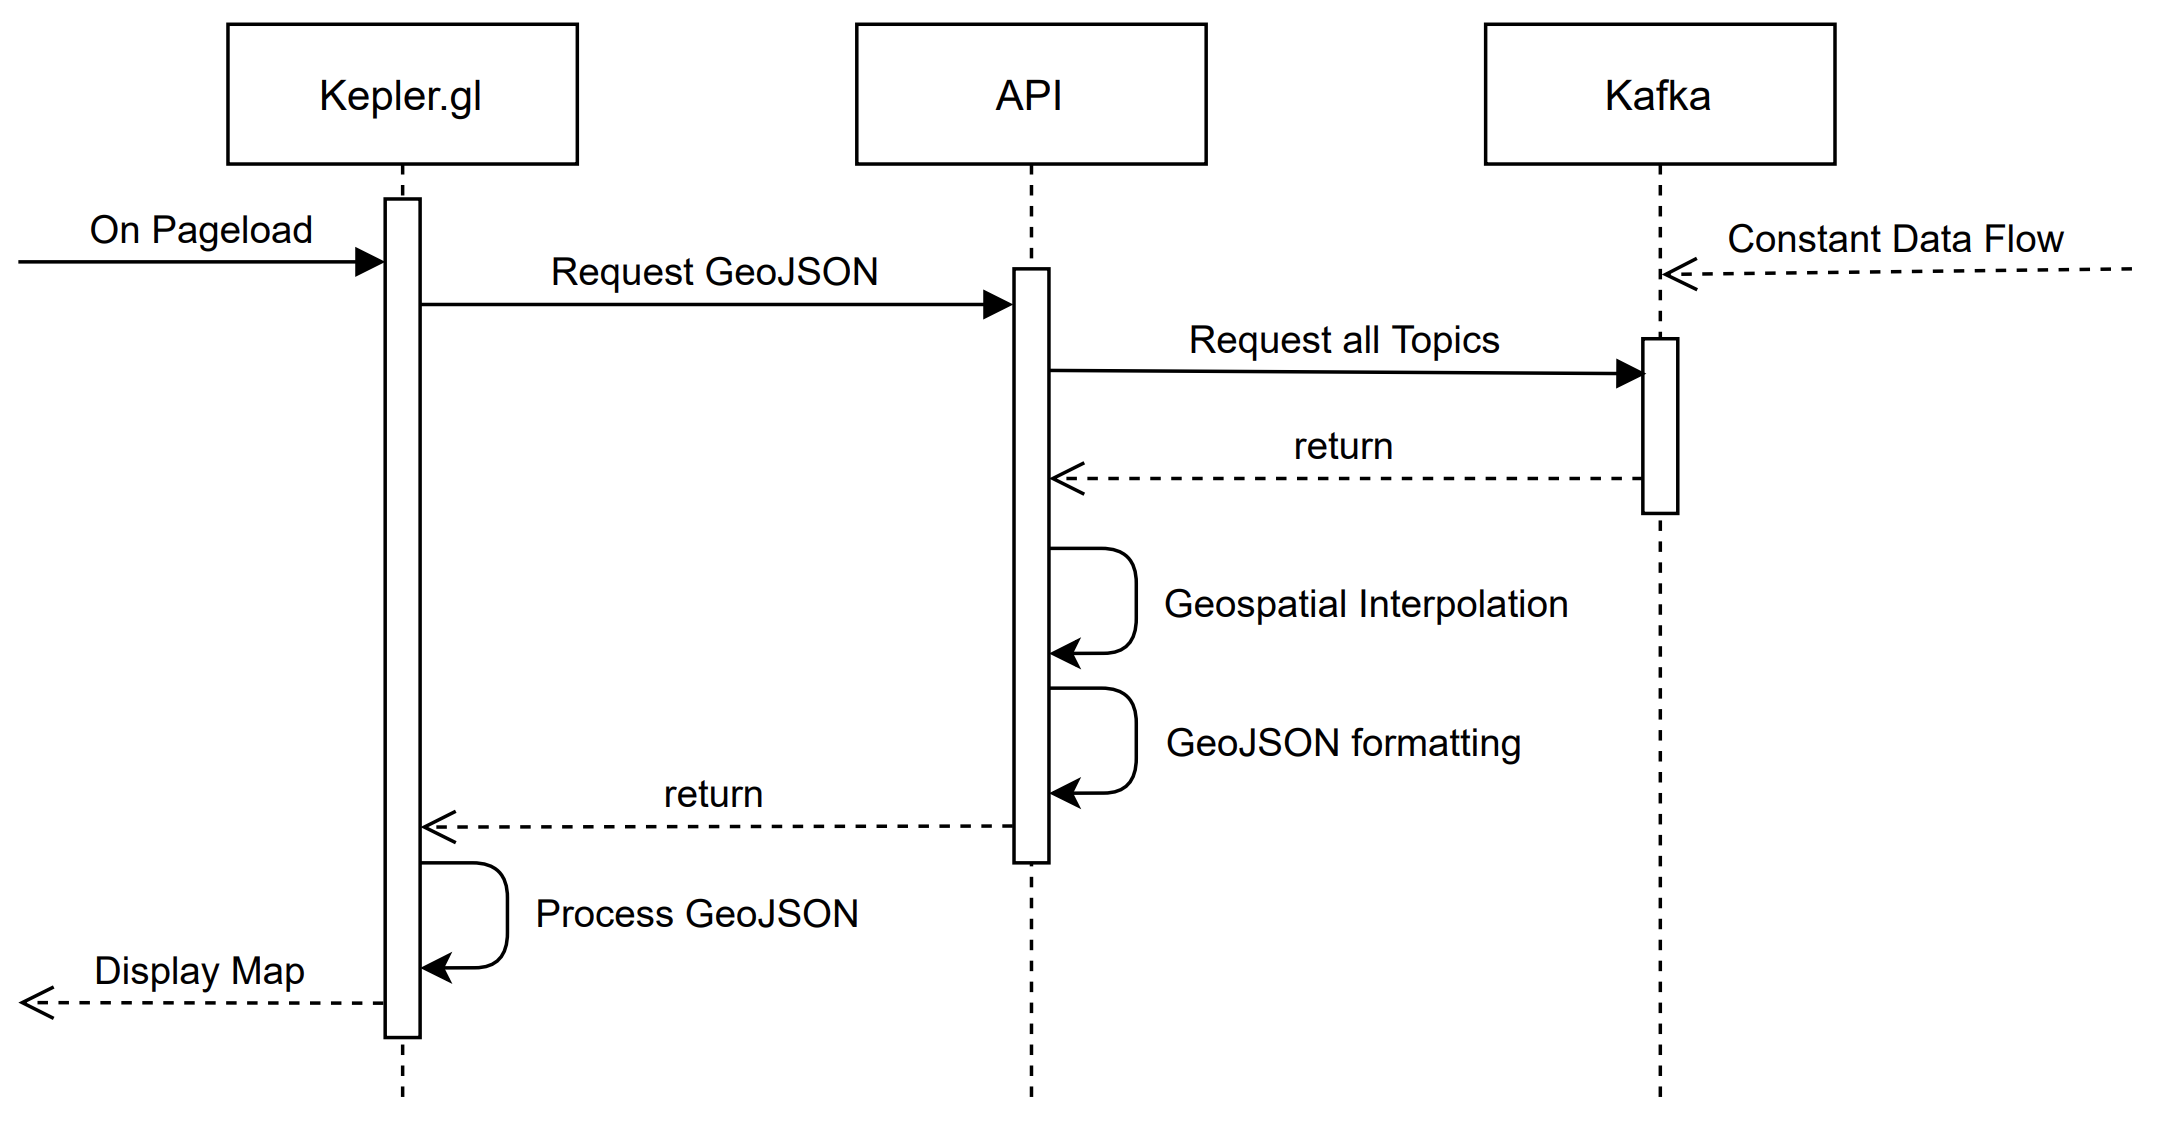
\includegraphics[width=.9\linewidth]{figures/Frontend_Flow.png}
\end{center}
\end{frame}

% hunter needs to work on wording in morning since he is tired
\begin{frame}{Geospatial Interpolation}
% Due hypothetical problem that there are a limited amount of data sources available over a geographical region (i.e. sparsity),
% at first, we will employ a interpolation model,
% but we will abstraction in place to employ more sophisticated models.
\begin{itemize}
    \item Interpolation over a geographical region fills sparsity
    \item Abstracted interpolation model object supports sophisticated methods
\end{itemize}
% acknowledge data availability issues make a more sophisticated model difficult (data vendor are not cheap)
\begin{center}
    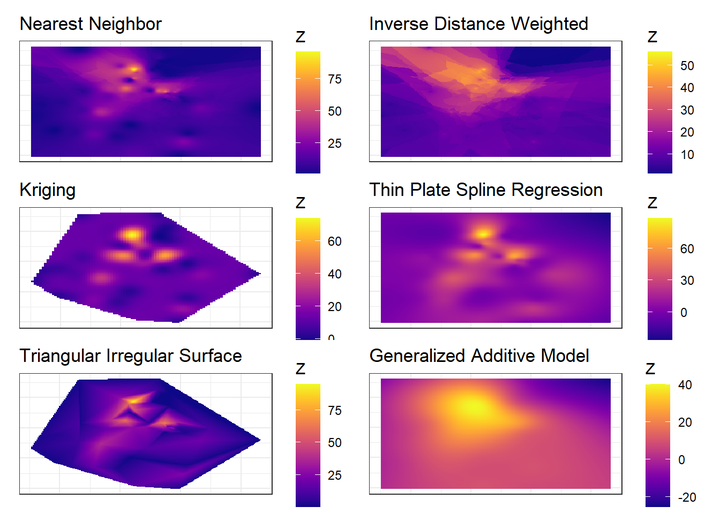
\includegraphics[width=0.7\linewidth]{figures/geostats.png} \\
\end{center}
\end{frame}

\begin{frame}{Visualization}
% incorporate something we learned in the class into this (IAC automation, containerization, elasticity, etc.)
\begin{itemize}
    % \item To visualize the results of interpolation, we are using kepler.gl, an open-source visualization tool developed specifically for geospatial data sets by Uber. 
    \item \textbf{Kepler.gl}, developed by Uber, is a powerful geospatial visualization tool
    \item React has libraries that support kepler.gl, making it possible to embed \textbf{live visualizations} in a react web-application.
\end{itemize}
\begin{center}
    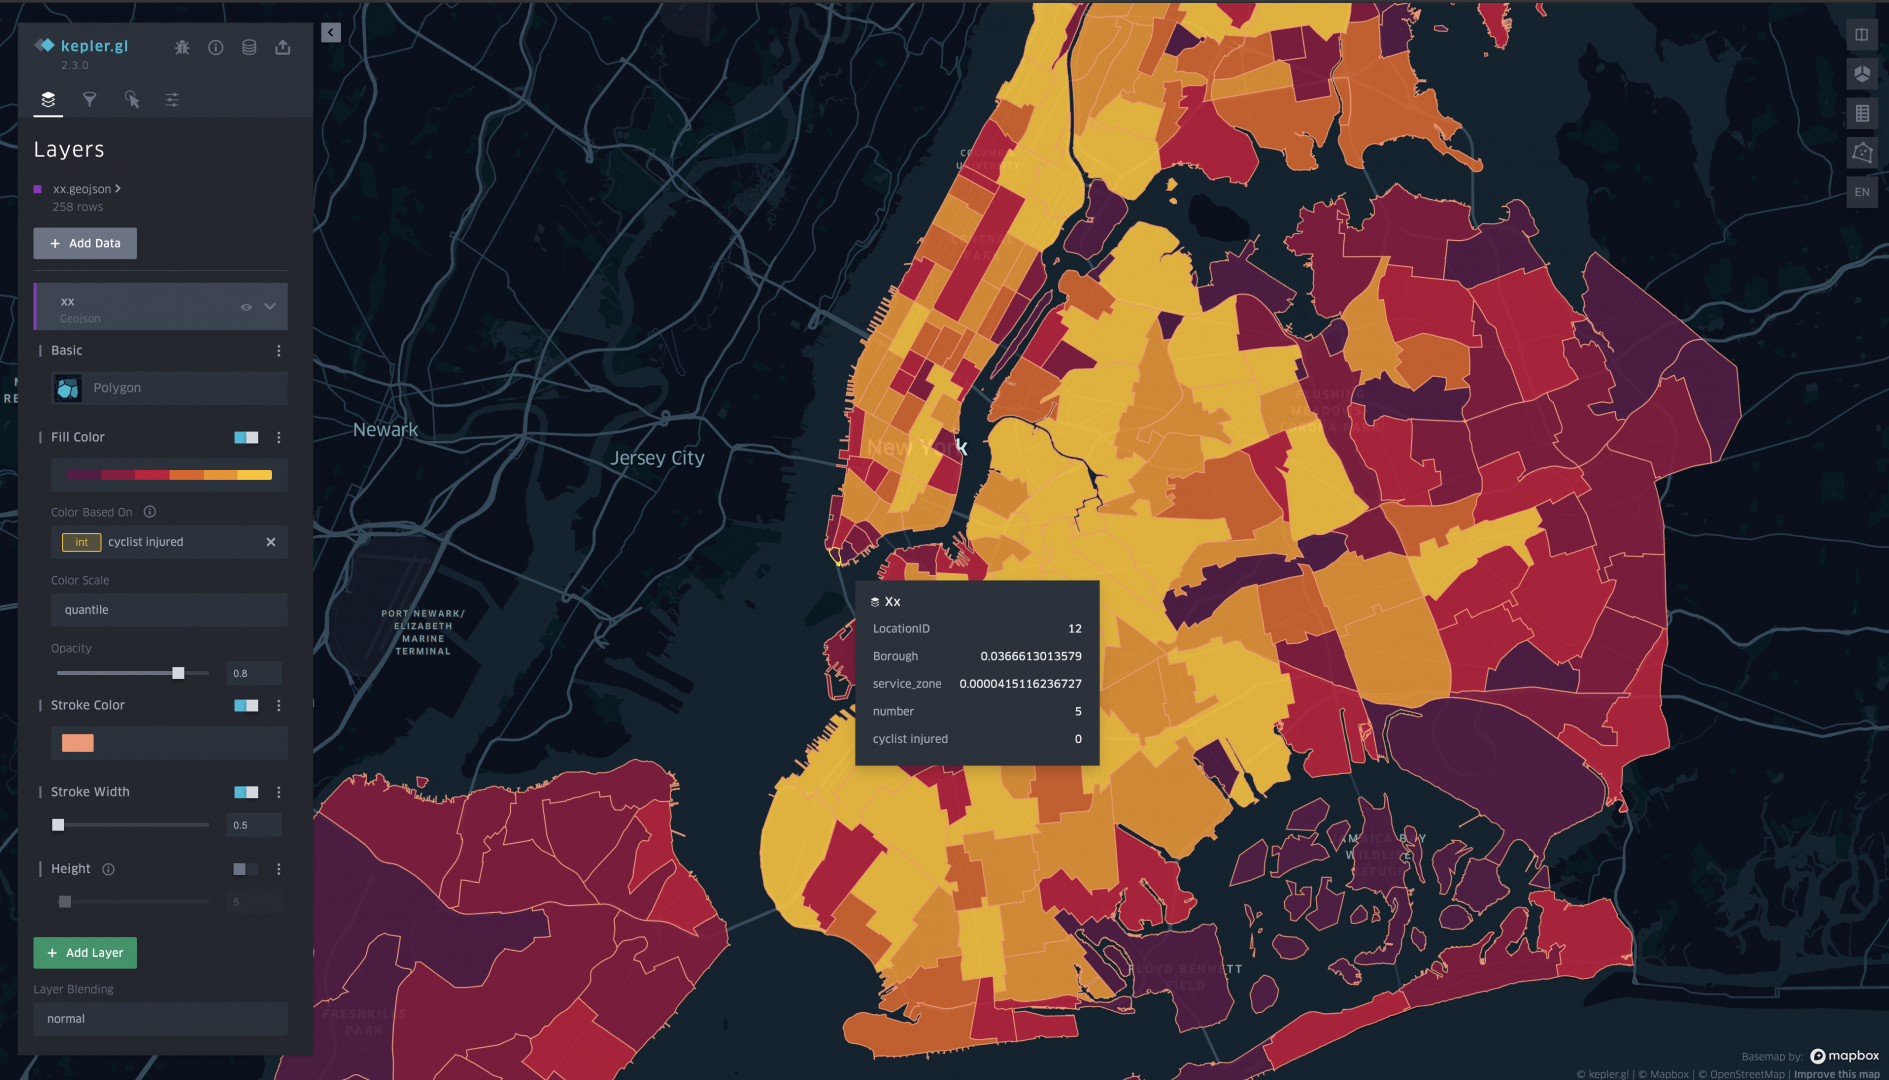
\includegraphics[width=0.60\linewidth]{documentation/project_presentation/figures/keplerpolygon.png} \\
\end{center}
\end{frame}

\end{document}